% THIS IS SIGPROC-SP.TEX - VERSION 3.1 WORKS WITH V3.2SP OF
% ACM_PROC_ARTICLE-SP.CLS APRIL 2009  It is an example file showing how to use
% the 'acm_proc_article-sp.cls' V3.2SP LaTeX2e document class file for
% Conference Proceedings submissions.
% ----------------------------------------------------------------------------------------------------------------
% This .tex file (and associated .cls V3.2SP) *DOES NOT* produce:
% 1) The Permission Statement 2) The Conference (location) Info information 3)
% The Copyright Line with ACM data 4) Page numbering
% ---------------------------------------------------------------------------------------------------------------
% It is an example which *does* use the .bib file (from which the .bbl file is
% produced).
% REMEMBER HOWEVER: After having produced the .bbl file, and prior to final
% submission, you need to 'insert'  your .bbl file into your source .tex file so
% as to provide ONE 'self-contained' source file.
%  Questions regarding SIGS should be sent to Adrienne Griscti --->
% griscti@acm.org  Questions/suggestions regarding the guidelines, .tex and .cls
% files, etc. to Gerald Murray ---> murray@hq.acm.org  For tracking purposes -
% this is V3.1SP - APRIL 2009

\documentclass{acm_proc_article-sp}
\usepackage{algorithmicx}
\usepackage[ruled]{algorithm}
\usepackage{algpseudocode}
\algrenewcommand\algorithmicindent{0.8em}%

\begin{document}

\title{Automatic Web Page Segmentation and Noise Removal for Structured
Extraction using Tag Path Sequences
% \titlenote{(Does NOT produce the permission block, copyright information nor
% page numbering). For use with ACM\_PROC\_ARTICLE-SP.CLS. Supported by ACM.}
}
% \subtitle{[Extended Abstract] \titlenote{A full version of this paper is
% available as \textit{Author's Guide to Preparing ACM SIG Proceedings Using
% \LaTeX$2_\epsilon$\ and BibTeX} at \texttt{www.acm.org/eaddress.htm}}}  You
% need the command \numberofauthors to handle the 'placement and alignment' of
% the authors beneath the title.
%  For aesthetic reasons, we recommend 'three authors at a time' i.e. three
% 'name/affiliation blocks' be placed beneath the title.
%  NOTE: You are NOT restricted in how many 'rows' of "name/affiliations" may
% appear. We just ask that you restrict the number of 'columns' to three.
%  Because of the available 'opening page real-estate' we ask you to refrain
% from putting more than six authors (two rows with three columns) beneath the
% article title.
% More than six makes the first-page appear very cluttered indeed.
%  Use the \alignauthor commands to handle the names and affiliations for an
% 'aesthetic maximum' of six authors.
% Add names, affiliations, addresses for the seventh etc. author(s) as the
% argument for the \additionalauthors command.
% These 'additional authors' will be output/set for you without further effort
% on your part as the last section in the body of your article BEFORE References
% or any Appendices.

\numberofauthors{2} %  in this sample file, there are a *total*
% of EIGHT authors. SIX appear on the 'first-page' (for formatting reasons) and
% the remaining two appear in the \additionalauthors section.
\author{
% You can go ahead and credit any number of authors here, e.g. one 'row of
% three' or two rows (consisting of one row of three and a second row of one,
% two or three).
%  The command \alignauthor (no curly braces needed) should precede each author
% name, affiliation/snail-mail address and e-mail address. Additionally, tag
% each line of affiliation/address with \affaddr, and tag the e-mail address
% with \email.
%  1st. author
\alignauthor Roberto Panerai Velloso\\
       \affaddr{Universidade Federal de Santa Catarina}\\
       \affaddr{Brazil}\\
       \email{rvelloso@gmail.com}
% 2nd. author
\alignauthor Carina F. Dorneles\\
       \affaddr{Universidade Federal de Santa Catarina}\\
       \affaddr{Brazil}\\
       \email{dorneles@gmail.com}
}
% There's nothing stopping you putting the seventh, eighth, etc.
% author on the opening page (as the 'third row') but we ask, for aesthetic
% reasons that you place these 'additional authors' in the \additional authors
% block, viz.

% Just remember to make sure that the TOTAL number of authors is the number that
% will appear on the first page PLUS the number that will appear in the
% \additionalauthors section.

\maketitle
\begin{abstract}
Web page segmentation and data cleaning are essential steps in structured web
data extraction. Identifying a web page main content region, removing what is
not important (menus, ads, etc.), can greatly improve the performance of the extraction
process. We propose, for this task, a novel and fully automatic algorithm that
uses a tag path sequence (TPS) representation of the web page. The TPS consists
of a sequence of symbols (string), each one representing a different tag path.
The proposed technique searches for positions in the TPS where it is possible to
split it in two regions where each region's alphabet do not intersect,
which means that they have completely different sets of tag paths and, thus, are
different regions. The results show that the algorithm is very effective in
identifying the main content block of several major websites, and improves the
precision of the extraction step by removing irrelevant results.
\end{abstract}

\category{H.2.8}{Database Management}{Database Applications}[Data mining] 
\category{H.3.3}{Information Storage and Retrieval}{Information Search and Retrieval}[Information filtering]
\category{I.1.2}{Symbolic and Algebraic Manipulation}{Algorithms}[Analysis of algorithms]

%\terms{Theory}

\keywords{noise removal, page segmentation, structured extraction, web mining}

\newdef{definition}{Definition}

\section{Introduction}  %Extensive research is still undergoing in the field of
web mining. Being the %WWW as vast as it is, with all kinds of transactions
taking place in it and %serving as backbone for enterprises and governments,
it's easy to see its %intrinsic value, proportional to the amount of information
it holds, mostly %hidden behind corporative web sites. To retrieve this
information, web mining %techniques are being developed for as long as the WWW
and the internet exists.  One crucial step in web data mining, including
structured extraction, is the cleaning phase that takes place before extracting
the information. One can not expect to get good results in the extraction phase
without cleaning and removing the undesired noise first.  %In
\cite{Editorial04}, it is mentioned that noise can seriously harm web data
mining. In \cite{Noisy03}, it is mentioned that despite the importance of this
task, relatively  little work has been done in this area and, while reviewing up
to date related work we  still have the impression, that this is an
underdeveloped field. Moreover, according to  \cite{Editorial04}, noise can
seriously harm web data mining.   In structured extraction, most of the existing
approaches use some sort of pattern recognition to identify the records (as
defined in \cite{MDR03}) present in the page. The problem is that, usually, we
are interested only in the main content region, as depicted in Figure
\ref{fig:ex2}, but other regions of the page (menus, ads, etc.) often contain
repeating patterns that are outputted as noise results. So, it is useful to
cleanup a web page before extracting the records from it.  Currently, some of
the works on noise removal and page segmentation are aimed at page indexing and
clustering (i.e. they assume the main region is textual) such as
\cite{SiteOriented11,Noisy03} and, due to intrinsic differences between
unstructured data and structured data, these can not be used for structured
extraction. The existing techniques that can be used for structured content
either require a priori definitions (\cite{vips03}), or prior training
(\cite{Graph08}) or they rely on specific HTML tags or aspects of the HTML
language to work, such as \cite{Entropy09}.  In this paper, we propose and lay
down a simple, computationally efficient, yet very powerful, algorithm aimed at
web page segmentation, noise removal and main content identification, based on
the tag path sequence of the web page. It is a general segmentation technique,
presented here in the context of structured extraction, that takes into account
the page's style and structure. Our main contributions are:
\begin{itemize} 
\item{Fully automatic}: no training or human
intervention needed; 
\item{Domain independent}: it is only required that a page
contains structured content, no matter what domain it is about; 
\item{HTML
syntax independent}: there are no rules defined for specific HTML tags; 
\item{Works on single page}: it is required only one page as input, which is a
main advantage as discussed in \cite{Editorial04}; 
\item{Can be combined with
extraction techniques}: due to the way pruning is carried out (preserving tree
structure), this algorithm can be combined with any structured extraction
algorithm; 
\item{Extraction optimization}: the proposed algorithm prunes and
average of 46.22\% of the DOM tree, in linear time, avoiding the processing of
this noise by the subsequent extraction algorithm.   
\end{itemize}
 
%To evaluate how effective our approach is, we compared the noise output of
%MDR \cite{MDR03}, a well known structured extraction technique, with and without
%the use of our technique, yielding and average of 77.03\% of noise removed from
%the test web pages.

To evaluate how effective our approach is, we have compared the output of
MDR \cite{MDR03}, a well known structured extraction technique, against the output
of MDR combined with our technique, as illustrated in Figure \ref{fig:method}, yielding 
and average of 77.03\% of noise removed from the test web pages.

\begin{figure}[H]
  \centering
    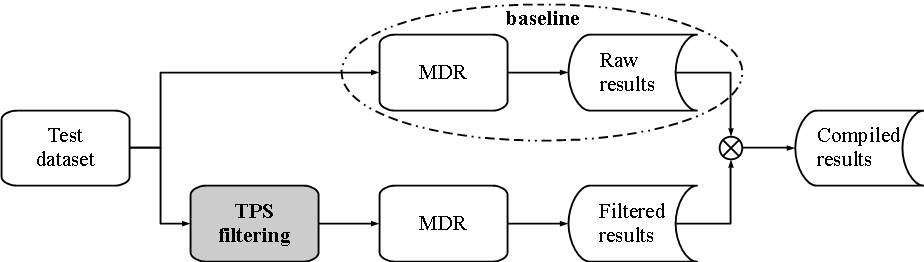
\includegraphics[scale=0.34]{method.jpg}
  \caption{Evaluation method adopted.}
  \label{fig:method}
\end{figure}
 
This paper is organized as follows. In Section \ref{sec:relatedwork}, we give a
brief survey of related works in segmentation, pointing out the differences
between each one and our proposal. In Section \ref{sec:basicdefs}, some basic
definitions are given, which are needed for the problem definition and the
understanding of the algorithm. In Section \ref{sec:probform}, we state the
problem and explain the two hypothesis that are the basis on which we develop
the proposed solution for the problem of segmentation and noise removal,
targeted at structured extraction. In Section \ref{sec:algorithm}, a detailed
description of the full algorithm and its complexity are given. In Section
\ref{sec:results}, we present the results of the tests done so far.
Finally, in Section \ref{sec:conclusion}, a conclusion is given and possible
future developments are outlined.

\section{Related Work}\label{sec:relatedwork}

There are several works proposing ways to segment web pages and identify what is
noise and what is informative content in them. We grouped them in three
different categories: those based on text content, those based on the DOM tree
and those that make use of visual information.

\textbf{Text content based approaches}. In
\cite{BlockImp07,Densiometric08,Boilerplate10,CETR10,NonTemplate13} the segmentation is done
using the text content of the web page. The focus of these works, however, is
not on structured extraction, but instead, on indexing and clustering of web
sites. The majority of the works about page cleaning and noise removal are aimed
at this kind of applications.

\textbf{DOM tree based approaches}. In
\cite{Noisy03,Graph08,Entropy09,SiteOriented11,Entropy12,Jointop07} the segmentation is done using
the DOM tree and, thus, they do take into account the web page's structure.
However \cite{SiteOriented11} and \cite{Noisy03} require several pages from the
same web site, they are site-driven techniques, \cite{Graph08} and \cite{Jointop07} proposes a
training framework that requires a manually labeled data set to work, \cite{Entropy09}
is dependent of a tag dictionary, defined a priori, to build a
visual representation of the page and \cite{Entropy12} requires a database of terms associated
to ``semantic roles'' in order to detect data-rich regions.

\textbf{Visual information based approaches}. Besides text and DOM tree
based techniques, there are the ones based on visual information such as
\cite{vips03,viper05,vide09}. They all rely on a web browser's renderer to
obtain the visual information used for segmentation, what can be
computationally expensive, and beyond that, \cite{vips03} is based on quite
a large set of strong heuristic rules, each one applied to specific HTML tags.
Approaches based on specific HTML tags have a serious disadvantage of being
affected by changes in web page design practices and HTML syntax changes.

\textbf{Structured extraction techniques}. There are a number of techniques 
proposed to address the problem of structured extraction, like 
\cite{NET05,RRunner01,MDR03,TPC09,SuffixTree12}, just to name a few. The reason we 
chose MDR for the evaluation of our proposal is due to the level of detail provided by the 
publications (which allows for implementation) and availability of independent implementations. 
Since we are measuring only the noise suppressed in the output, and not the quality of the extraction itself, 
any pattern detection algorithm, that complies with our constraints (fully automatic, 
works on single page, no training, no labeling, etc.), would suffice.   

The representation of the web page used in our work (tag path sequence) was
also employed in \cite{TPC09} and \cite{SuffixTree12}, although in both cases
for structured extraction, not for segmentation. We cite them here to show
that, according to their results, this representation, just like the DOM tree,
is also able to expose the web page's structure and, thus, is suitable for the
purpose of our work.

\section{Basic Definitions}\label{sec:basicdefs}

Now we present the concepts and definitions used to state the problem in
Section \ref{sec:probform} and outline the proposed algorithm in Section
\ref{sec:algorithm}, as well as an example to illustrate each definition.

\begin{definition}\textbf{(DOM tree).}\label{def:domtree}
The DOM tree is a hierarchical structure,
derived from the parsing of HTML code, that represents a web page.
\end{definition}
In Figure \ref{fig:ex1} we use a small piece of HTML code to illustrate the
DOM tree and the next definitions.

\begin{definition}\textbf{(Tag path).}\label{def:tp} A tag path ($TP$) is a
string describing the absolute path from the root of the DOM tree to a given
node. Let $i$ be the depth-first position, in the DOM tree, of a $node_i$, then
we say that the tag path $TP_i$ is a string describing the path from the root of the
DOM tree to the $node_i$.
\end{definition}
In Figure \ref{fig:ex1}, the absolute tag path $TP_4$ from the
node $body$ to the table cell node $td_4$ is $TP_4=``body/table/tr/td"$.

\begin{definition}\textbf{(Tag path sequence).}\label{def:tps} We define the tag
path sequence ($TPS$) of a DOM tree with $n$ nodes to be the ordered sequence
$TPS[1..n] = (TP_1,TP_2,TP_3, ...,TP_{n-1},TP_n)$ where two tag paths $TP_i$
and $TP_j$, with $i\neq{}j$, are considered equal only if their paths and
style definitions are equal, otherwise they are different.
\end{definition}
This is the same definition as in \cite{SuffixTree12}, where each different tag
path is represented in the sequence by a symbol, except that here we incorporate
style definitions when comparing tag paths. In Figure \ref{fig:ex1} we show the
$TPS$ for the given HTML code, where each $TP$ is assigned a code,
yielding $TPS = (1,2,3,4,4,3,4,4)$.

\begin{definition}\textbf{(Alphabet of the TPS).}\label{def:alpha} Let $\Sigma_a$
be a set containing all the symbols in a given sequence $TPS_a$ of size $n$, we say that
$\Sigma_a$ is the alphabet of $TPS_a$ defined as $\Sigma_a = \{\alpha |
\exists{TPS_a[i]}=\alpha \wedge 1 \leq i \leq n\}$, where $\alpha$ is a symbol
in the alphabet.
\end{definition}
Informally speaking, the alphabet indicates all distinct symbols in a $TPS$. In
Figure \ref{fig:ex1}, the $TPS$ is formed only by the symbols ``1'',``2'', ``3''
and ``4'', so its alphabet is $\Sigma=\{1,2,3,4\}$.

\begin{definition}\textbf{(Tag path frequency set).}\label{def:tpfs} Let
$(s,f)$ be a pair where $s$ is a symbol from an alphabet of
a given $TPS$ and $f$ is the number of times that $s$ appears in the $TPS$,
so we define the tag path frequency set as the set containing all possible
$(s,f)$ pairs of a $TPS$. Let $FS =
\{(s_1,f_{s1}),(s_2,f_{s2}),(s_3,f_{s3}),\ldots,(s_{n-1},f_{sn-1}),(s_n,f_{sn})\}$,
where $n$ is the size of the $TPS$.
\end{definition}
In Figure \ref{fig:ex1}, symbol ``1'' shows up once in the sequence,
symbol ``2'' once too, symbol ``3'' twice and symbol ``4'' four times, so
for this sequence the tag path frequency set is equal to $FS = \{(1,1), (2,1), \\
(3,2), (4,4)\}$. The set $FS$ is a mapping between every symbol of an alphabet
an its corresponding frequency.

\begin{definition}\textbf{(Frequency thresholds).}\label{def:ft} Given a $TPS_a$
with alphabet $\Sigma_a$, tag path frequency set $FS_a$, we define the frequency
thresholds $FT_a$ to be the ordered set containing only the frequencies of $FS_a$.
Let $FT_a = \{f|\exists{(s,f)} \wedge (s,f) \in FS_a \wedge s \in \Sigma_a \}$, where $f$
is a frequency, $s$ is the corresponding symbol of the alphabet $\Sigma_a$.
\end{definition}

In the TPS from Figure \ref{fig:ex1}, the tag path frequency set is 
$FS=\{(1,1), (2,1), (3,2), (4,4)\}$, in this case the frequency thresholds is
equal to $FT=\{1,2,4\}$ because symbols ``1'' and ``2'' both have frequency
equal \textbf{1}, symbol ``3'' has frequency equal \textbf{2} and symbol ``4''
has frequency equal \textbf{4}. The $FT$ set is need to filter out
symbols from the $TPS$. If we have a set $FT=\{1,2,4\}$, there is no point in
filtering symbols with $f=3$, because there is none in the sequence.

\begin{definition}\textbf{(Region).}\label{def:region} Let a tag path sequence
$TPS$ be a concatenation of two other sequences $TPS=TPS_a . TPS_b$, we say that $TPS_a$
and $TPS_b$ are regions of $TPS$, iff $\Sigma_a \cap \Sigma_b = \emptyset$.
\end{definition}
In Figure \ref{fig:ex1} if we divide the TPS in two subsequences
$TPS_a=TPS[1..2]=(1,2)$ and $TPS_b=TPS[3..8]=(3,4,4,3,4,4)$, with alphabets
$\Sigma_a=\{1,2\}$ and $\Sigma_b=\{3,4\}$, we say that $TPS_a$ and $TPS_b$ are
distinct regions of $TPS$, because $\Sigma_a \cap \Sigma_b=\emptyset$.

\begin{figure}[H]
  \centering
    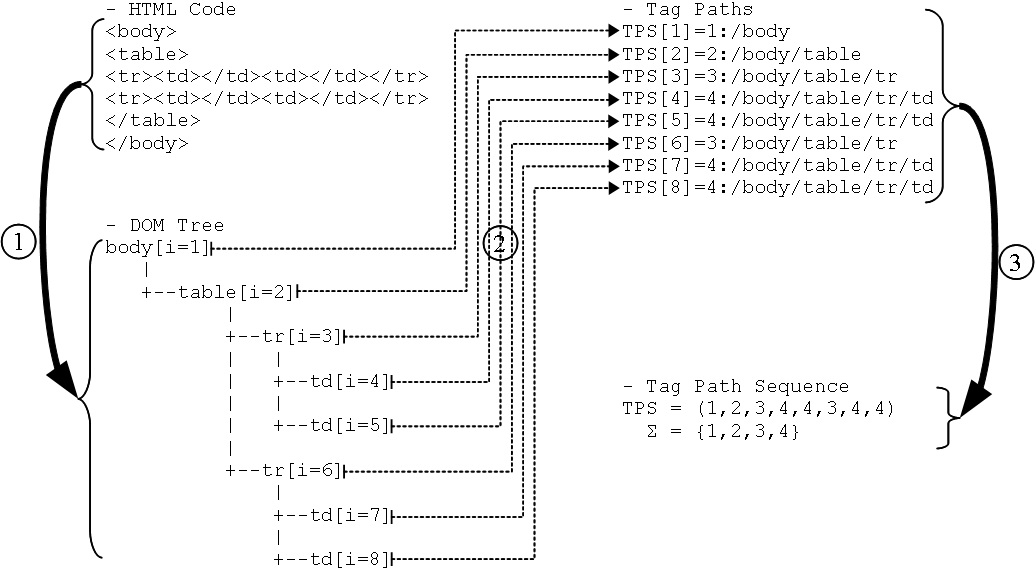
\includegraphics[scale=0.30]{example1.jpg}
  \caption{An example of a TPS being built from an HTML code.}
  \label{fig:ex1}
\end{figure}

%\subsection{Example}
%\begin{itemize}
%\item{HTML Code}:
%\begin{verbatim}
%<body>
%<table>
%<tr><td></td><td></td></tr>
%<tr><td></td><td></td></tr>
%</table>
%</body> 
%\end{verbatim}

%\item{DOM tree}
%\begin{verbatim}
%body[i=1]
%   |
%   +--table[i=2]
%          |
%          +--tr[i=3]
%          |   |
%          |   +--td[i=4]
%          |   |
%          |   +--td[i=5]
%          |
%          +--tr[i=6]
%              |
%              +--td[i=7]
%              |
%              +--td[i=8]
%\end{verbatim}

%\item{Tag paths}
%\begin{verbatim}
%TPS[1]=1:/body
%TPS[2]=2:/body/table
%TPS[3]=3:/body/table/tr
%TPS[4]=4:/body/table/tr/td
%TPS[5]=4:/body/table/tr/td
%TPS[6]=3:/body/table/tr
%TPS[7]=4:/body/table/tr/td
%TPS[8]=4:/body/table/tr/td
%\end{verbatim}

%\item{Tag path sequence}
%\begin{verbatim}
%TPS = (1,2,3,4,4,3,4,4)
%\end{verbatim}
%\end{itemize}

\section{Problem formulation}\label{sec:probform}
Given the definitions presented in the previous section, we formulated the
problem of page segmentation and noise removal, based on the following
assumptions:

\begin{enumerate}
\item\label{ass:1}
different regions of a web page are described using different tag paths, so
these regions will have different alphabets; and
\item\label{ass:2}
in web sites with semi-structured content (i.e. records, as defined in
\cite{MDR03}), the main region is structurally denser than the others (menus, ads,
text, etc.).
\end{enumerate}

The basis for assumption (\ref{ass:1}) comes from the observation that the
regions of a web page are different ramifications in the DOM tree and these
regions are described either using different tags for each one or, if the tags
are the same, with different styles, so that they can easily be distinguished by
the user. If all regions of a page look alike, it gets more
difficult, for the user, to tell them apart. Then, from Definition \ref{def:tps}
we can see that the set of symbols used in each region of a web page should be
different, and so it should be possible to segment a page using Definition
\ref{def:region}.

The assumption (\ref{ass:2}) comes from the context in which we apply the page
segmentation proposed in this work (i.e. structured extraction). Since
we are segmenting only pages containing records, and we know that in order
to describe the structure of these records, in HTML, we need more nodes of the DOM
tree than for unstructured data (i.e. text), it is reasonable to assume that,
for a page containing records, the main region is the largest one (i.e. the
one with more nodes).

Now, using the definitions in Section \ref{sec:basicdefs} and the above
assumptions, we can state the problem of web page segmentation and
main content identification to be the following: \textbf{``find the largest
$region$ in the $TPS$ of a web page that has an $alphabet$ that do not intersect
with the $alphabet$ of other smaller regions''}.

One \textbf{crucial} detail that has to be taken into account, is that there may
be tag paths in a page that represent structural divisions of it (i.e. web
site's visual formatting). These tag paths, if they are divisions, will show up
a few times throughout the entire sequence, preventing us from finding a split,
in the TPS, where the alphabets of the two parts of the sequence do not intersect.
To remove this $noise$ from the TPS, we filter out, iteratively, all symbols
with lower frequencies. This way we can avoid this problem without harming the
segmentation process, because the tag paths with higher frequencies are still
being considered.

For illustration purposes, we give now an example of a web page starting
and ending with the same tag path (``/body/br'') and with three regions
delimited by the same tag path (``/body/div''). Assuming that different tag
paths are used to describe each region, without filtering out low frequency tag
paths from the $TPS$ it would not be possible to split the sequence into regions.

\begin{itemize}
\item{HTML code}
\begin{verbatim}
<body>
   <br>
   <div>
      <span class='region1'></span>
      ...
      <span class='region1'></span>
   </div> 
   <div>
      <span class='region2'></span>
      ...
      <span class='region2'></span>
   </div> 
   <div>
      <span class='region3'></span>
      ...
      <span class='region3'></span>
   </div>
   <br>
</body>
\end{verbatim}
\item{TPS}
\begin{verbatim}
TPS = (1,2,3,4,...,4,3,5,...,5,3,6,...,6,2)
\end{verbatim}

The symbols $2$ and $3$ appear along the entire $TPS$.

\item{Filtered TPS}
\begin{verbatim}
TPS = ( , , ,4,...,4, ,5,...,5, ,6,...,6, )
\end{verbatim}

Only symbols with frequency higher than $3$ are considered in the segmentation
process. Now it is possible to split the $TPS$ into regions.

\end{itemize}
 
\section{Algorithm's description}\label{sec:algorithm}

In this section we present the algorithms we have developed to address the
problem stated in Section \ref{sec:probform}. They are the following:
\begin{itemize}
  \item {}\textit{\textbf{tagPathSequenceFilter()}}. It is the main algorithm, which
  receives a HTML file as input and returns a pruned DOM tree with the main content region;
  \item {}\textit{\textbf{convertToSeq()}}. It converts the web page DOM tree into a tag path sequence;
  \item {}\textit{\textbf{searchRegion()}}. It is the actual search for the main
  region of the TPS;
  \item {}\textit{\textbf{filter()}}. It filters an alphabet, removing lower
  frequency symbols, making the overall algorithm more robust and resistant to noise;
  \item {}\textit{\textbf{pruneDOMTree()}}. It prunes the original DOM tree, leaving only
  the main content region reported by $searchRegion$, keeping the original structure of the document.
\end{itemize}

\subsection{$tagPathSequenceFilter()$ Algorithm}

\begin{algorithm}[H]
\caption{Filters out noise from a web page}
\label{alg:tpsfilter}
\textbf{Input:} $inputFile$ - an HTML file \\
\textbf{Output:} pruned $inputFile$'s DOM tree
\begin{algorithmic}[1]
\Procedure{tagPathSequenceFilter}{$inputFile$}
\State $DOMTree \leftarrow parseHTML(inputFile)$
\State $convertToSeq(DOMTree.body,$`` ''$,TPS)$
\State $searchRegion(TPS)$
\State $pruneDOMTree(DOMTree.body,TPS)$
\State return $DOMTree$
\EndProcedure
\end{algorithmic}
\end{algorithm}

The procedure $tagPathSequenceFilter()$ in Algorithm \ref{alg:tpsfilter} returns
the main content region of $inputFile$. The procedure $parseHTML()$, in
Line $2$, converts the HTML code into a DOM tree representation;
$convertToSeq()$, in Line $3$, converts the DOM tree into a TPS; The
procedure $searchRegion()$, in Line $4$, recursively searches for the largest part
of the TPS that has a unique alphabet and, finally; $pruneDOMTree()$, in Line
$5$, prunes out of the DOM tree every node that is not in the resulting TPS,
preserving the structure of the returned document in Line $6$.

Bellow we detail the algorithms $convertToSeq()$, $searchRegion()$,
$filter()$ and $pruneDOMTree()$. The algorithm $parseHTML()$ is not in
the scope of our work and so, will not be discussed here.

\subsection{$convertToSeq()$ Algorithm}

\begin{algorithm}[H]
\caption{Converts a DOM tree to a tag path sequence representation}
\label{alg:tree2seq}
\textbf{Input:} $node$ - a DOM tree node, initially the root \\
\textbf{Input:} $tp$ - the previous tag path, initially empty \\
\textbf{Input:} $TPS$ - the $TPS$ built from the DOM tree,
initially empty \\
\textbf{Output:} the $TPS$ for the given DOM tree stored in $TPS$
\begin{algorithmic}[1]
\Procedure{convertToSeq}{node,tp,TPS by ref.}
\State $tp \leftarrow concat(tp,$``/''$,node.tag,node.style)$
\If {$tp \ni tagPathMap$}
\State $tagPathMap \leftarrow tagPathMap + \{tp\}$
\State $tagPathMap[tp].code \leftarrow tagPathMap.size$
\EndIf
\State $TPS \leftarrow concat(TPS,tagPathMap[tp].code);$
\For {each $child$ of $node$}
\State $convertToSeq(child,tp,TPS)$
\EndFor
\EndProcedure
\end{algorithmic}
\end{algorithm}

The procedure $convertToSeq()$ in Algorithm \ref{alg:tree2seq}
converts a web page from its DOM tree representation to a TPS representation,
traversing the DOM tree in depth-first order. It is initially called in
Algorithm \ref{alg:tpsfilter} with an empty $tagPath$ parameter, which
represents the previous tag path string (from the previous recursive call).
In Line $2$, the previous tag path is concatenated with the current tag, as well
as with its style definition, in order to distinguish repeated paths with different
styles; in Line $3$, it is checked whether or not the current tag path has been
seen before ($tagPathMap$ is used for this purpose) and, if not, in Line $4$, it 
is inserted into the set $tagPathMap$ and a new code assigned to it in Line $5$,
as stated in Definition \ref{def:tps}; in Line $7$, the tag path code is appended
to the end of the sequence and, finally, the procedure is called recursively in 
Line $9$ for each child of $node$.

\subsection{$searchRegion()$ Algorithm}

This is the core algorithm, since it is responsible for finding the main content region, 
so we have provided na illustration, in Figure \ref{fig:alg}, to help understand its workings. 
In Figure \ref{fig:alg}, for clarity purposes, we have omitted alphabet filtering in order 
to keep it simple and easy to understand the main idea behind $searchRegion()$ algorithm.

\begin{figure}[H]
  \centering
    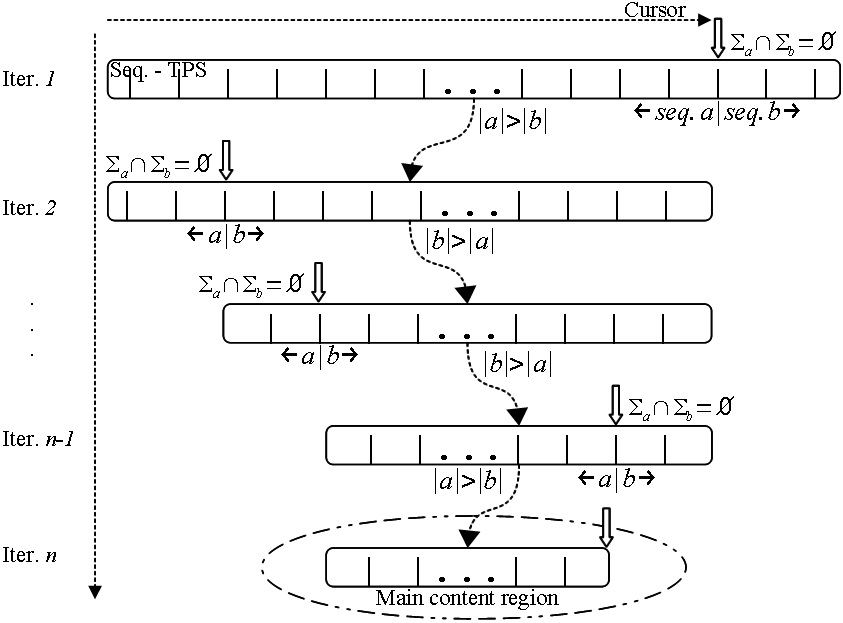
\includegraphics[scale=0.37]{alg-pb.jpg}
  \caption{Illustration of procedure $searchRegion()$.}
  \label{fig:alg}
\end{figure}

\begin{algorithm}[H]
\caption{Search for regions in the TPS with different alphabets}
\label{alg:searchreg}
\textbf{Input:} $TPS$ - the $TPS$ of a given page \\
\textbf{Output:} the main region of the $TPS$, stored in $TPS$
\end{algorithm}
\begin{algorithmic}[1]
\Procedure{searchRegion}{$TPS[1..n]$ by reference}
\State $\Sigma \leftarrow \emptyset$ \Comment alphabet
\State $t \leftarrow 0$
\For {$i \leftarrow 1..n$} \label{line:symfreq}
\State $sym \leftarrow TPS[i]$
\If {$sym \ni \Sigma$}
\State $\Sigma \leftarrow \Sigma \cup \{sym\}$
\State $symCount[sym] \leftarrow 0$
\EndIf
\State $symCount[sym] \leftarrow symCount[sym]+1$
\EndFor \label{line:esymfreq}
\State $thresholds \leftarrow OrderedFrequencySet(symCount)$ \label{line:freqth}
\State $regionFound \leftarrow false$
\While {not $regionFound$}\label{line:while}
\State $t \leftarrow t + 1$ \label{line:freqit}
\State $cur\Sigma \leftarrow filter(\Sigma,symCount,thresholds[t])$ \label{line:filter}
\If {$cur\Sigma.size < 2$}
\State $break$
\EndIf
\State $curSymCount \leftarrow symCount$
\State $region\Sigma \leftarrow \emptyset$
\State $gapSize \leftarrow 0$
\For {$i \leftarrow 1..n$} \label{line:tpsit}
\State $sym \leftarrow TPS[i]$
\If {$sym \in cur\Sigma$}
\State $region\Sigma \leftarrow region\Sigma \cup \{sym\}$ \label{line:regalpha}
\State $curSymCount[sym] \leftarrow curSymCount[sym] - 1$
\If {$curSymCount[sym] = 0$} \label{line:reg}
\State $cur\Sigma \leftarrow cur\Sigma - \{sym\}$
\If {$cur\Sigma \cap region\Sigma = \emptyset$}
\State $sizeRatio \leftarrow (n-2*i+gapSize)/n-gapSize$
\If {$cur\Sigma \neq \emptyset$ and $sizeRatio > 0.20$}
\State $regionFound \leftarrow true$
\State $break$
\Else
\State $gapSize \leftarrow 1$ 
\EndIf
\EndIf
\EndIf \label{line:ereg}
\Else
\If {$gapSize > 0$}
\State $gapSize \leftarrow gapSize+1$
\EndIf 
\EndIf
\EndFor
\EndWhile \label{line:ewhile}
\If {$regionFound$} \label{line:split}
\If {$i < n/2$}
\State $TPS \leftarrow TPS[i+1..n]$
\Else
\State $TPS \leftarrow TPS[1..i]$
\EndIf
\State $searchRegion(TPS)$ \label{line:recur}
\EndIf \label{line:esplit}
\EndProcedure
\end{algorithmic}
%\end{algorithm}

The procedure $searchRegion()$ in Algorithm \ref{alg:searchreg} computes the TPS
alphabet and corresponding symbol frequency from Lines \ref{line:symfreq} to
\ref{line:esymfreq}; in Line \ref{line:freqth}, the frequency thresholds, from
Definition \ref{def:ft}, are computed; from Lines \ref{line:while} to
\ref{line:ewhile} the actual search is performed for a position in the TPS where
a split is possible (i.e. where a region exists); in Line \ref{line:freqit} the
frequency thresholds are iterated; in Line \ref{line:filter} the TPS alphabet,
from Definition \ref{def:alpha}, is filtered, as described in Section
\ref{sec:probform};  in Line \ref{line:tpsit} the TPS is iterated; in Line
\ref{line:regalpha} the region alphabet is computed and;  from Lines
\ref{line:reg} to \ref{line:ereg} it is checked if there is no intersection
between the alphabets  of the two portions of the TPS (an empty intersection
indicates that a possible region was found, as in Definition \ref{def:region}).
The found region is only reported if it is at least $20\%$ larger than the rest
of the sequence, otherwise we continue iterating the sequence and the frequency 
thresholds. This percentage is actually a parameter and its purpose is to avoid reporting a
region under ambiguous conditions (in the experiments we used the value of
20\%); the purpose of variable $gapSize$ is to control the gap of low frequency symbols 
between two regions when they are not large enough to be reported; finally from Lines \ref{line:split} to \ref{line:esplit} the  TPS is
split if a region was found, calling $searchRegion()$ recursively in line
\ref{line:recur}, if so.

\subsection{$filter()$ Algorithm}

\begin{algorithm}[H]
\caption{Filters out symbols with lower frequencies from the alphabet}
\label{alg:filteralpha}
\textbf{Input:} $\Sigma$ - the alphabet ot be filtered \\
\textbf{Input:} $symCount$ - the tag path frequency set ($FS$) of $\Sigma$ \\ 
\textbf{Input:} $threshold$ - a frequency threshold \\
\textbf{Output:} a filtered alphabet
\begin{algorithmic}[1]
\Procedure{filter}{$\Sigma$, symCount, threshold}
\State $filtered\Sigma \leftarrow \emptyset$
\For {$i \leftarrow 1..n$}
\If {$symCount[\Sigma[i]] \geq threshold$}
\State $filtered\Sigma \leftarrow filtered\Sigma \cup \{\Sigma[i]\}$
\EndIf
\EndFor
\State return $filtered\Sigma$
\EndProcedure
\end{algorithmic}
\end{algorithm}

The procedure $filter()$ in Algorithm \ref{alg:filteralpha} removes from
alphabet $\Sigma$, every symbol with frequency lower than $threshold$. in Lines $3$ to
$7$ only the symbols with frequency greater or equal to $threshold$ are inserted
in the resulting set. The result of $filter()$ is used in Algorithm 
\ref{alg:searchreg}, Line $24$, where only the symbols in $filtered$ are
considered while searching for a region.

\subsection{$pruneDOMTree()$ Algorithm}

\begin{algorithm}[H]
\caption{Prune from the DOM tree the nodes that are not in sequence}
\label{alg:prune}
\textbf{Input:} $node$ - a DOM tree node, initially the root \\
\textbf{Input:} $seq$ - the TPS that has to remain in the DOM tree \\
\textbf{Output:} the DOM tree pointed by $node$ pruned
\begin{algorithmic}[1]
\Procedure{pruneDOMTree}{$node$ by ref.,$seq$}
\For {each child of node}
\If {$pruneDOMTree(child,seq) = true$}
\State remove child from $node$
\EndIf
\EndFor
\If {$node \ni seq$ and $node.childCount = 0$}
\State return $true$
\EndIf
\State return $false$
\EndProcedure
\end{algorithmic}
\end{algorithm}

The procedure $pruneDOMTree()$ in Algorithm \ref{alg:prune}, traverses the DOM
tree, depth first, removing the nodes that do not belong to $sequence$. In Line
$3$ the DOM is traversed; in Lines $7$ to $9$ it is decided whether or not
$node$ should be removed.

A node is removed from the tree, only if it is not in $sequence$ \textbf{and} has no children. 
This way we keep the structure of the remaining tree intact, in order not to affect the subsequent 
structured extraction phase.

\subsection{Algorithm's complexity}

As for the algorithm's complexity, if we observe Lines $14$ and $22$ of the
procedure $searchRegion()$, we can see that the loop in Line $14$ iterates the
frequency thresholds until a region is found and Line $22$ iterates the TPS
(filtered at given frequency threshold) also until a region is found and, if
so, the reported region is recursively processed.

In the worst case, when the alphabet intersection is empty only in the last
index of the TPS, the complexity would be at most $O(n^2 f)$, where $n$ is the
length of the TPS and $f$ is the size of the set $thresholds$. In practice, the
size of the set $thresholds$ is much smaller than the length of the TPS, so we
can say the complexity approximates $O(n^2)$ as shown in Equation \ref{eq:w}.
  \begin{equation}\label{eq:w}
  T(n) = T(n - 1) + \Theta(n) \Longrightarrow \sum_{i=1}^{n}
  i = \frac{n(n+1)}{2} = O(n^2)
  \end{equation} 

In average, if the TPS gets split in half, the complexity would be $O(n)$ as in
Equation \ref{eq:a}.
  \begin{equation}\label{eq:a}
  T(n) = T(n/2) + \Theta(n) \Longrightarrow \sum_{i=1}^{log_{2}^{n}}
  \frac{n}{2^i} = n - 1 = O(n)
  \end{equation} 

In the best case, TPS is split in the first index, yielding $O(n)$ as in
Equation \ref{eq:b}.
  \begin{equation}\label{eq:b}
  T(n) = T(n - 1) + \Theta(1) \Longrightarrow \sum_{i=1}^{n} 1 = n = O(n)
  \end{equation} 

In real world scenarios, as we have seen while doing the evaluation of the
algorithm, the sequences get split approximately four of five times until they
can not be split no more. So we can say that in real cases, the algorithm executes in
$O(in)$ time, where $n$ is the size of the $TPS$ and $i$ is the number of times the 
sequence gets split, which we can consider as a small constant, in this case, and 
say that it runs in $O(n)$.

\section{Experimental Results}\label{sec:results}

In this section we describe and discuss the results of our experiments and how
they are presented. To obtain the results presented in Subsection \ref{sub:res}, 
we have implemented the algorithm and tested it against some commercial and 
institutional web sites. In Subsection \ref{sub:clar} we detail one of the results 
presented, as an example, to clarify how they are compiled in Table \ref{table:results}.

\subsection{Experimental setup}\label{sub:clar}

We considered the extraction results of MDR alone as our baseline to be compared with
the results obtained by the combined use of TPS filtering and MDR, as illustrated in Figure \ref{fig:method}.

When applying both approaches (MDR and TPS filtering+MDR) to a result page of YouTube web site, the following 
results are obtained:

\begin{itemize}
\item{}raw web page (i.e. the original page, without TPS filtering)
\begin{itemize}
\item{}DOM tree processed: $1424$ nodes;
\item{}MDR results: $82$ records total ( $62$ noise / $20$ targets );
\end{itemize}

\item{}pruned web page (i.e. the web page after TPS filtering)
\begin{itemize}
\item{}DOM tree processed: $674$ nodes, size $47,33\%$ of the original page, reduction of $(-52,67\%)$
\item{}MDR results: $20$ records total ( $0$ noise / $20$ targets ), noise
removed $100\%$
\end{itemize}
\end{itemize}

In this result, we can see an improvement in the extraction of
records as well as a considerable reduction in the size of the DOM tree to be processed. 
A percentage of $52.67\%$ of the DOM tree was pruned without losing the
target records in the process. Everything pruned out of the DOM tree was noise. 
Figure \ref{fig:ex2} illustrates the web page and the main content region and in 
Figure \ref{fig:tps} we show the respective TPS and main content region detected by our algorithm.

\begin{figure}[H]
  \centering
    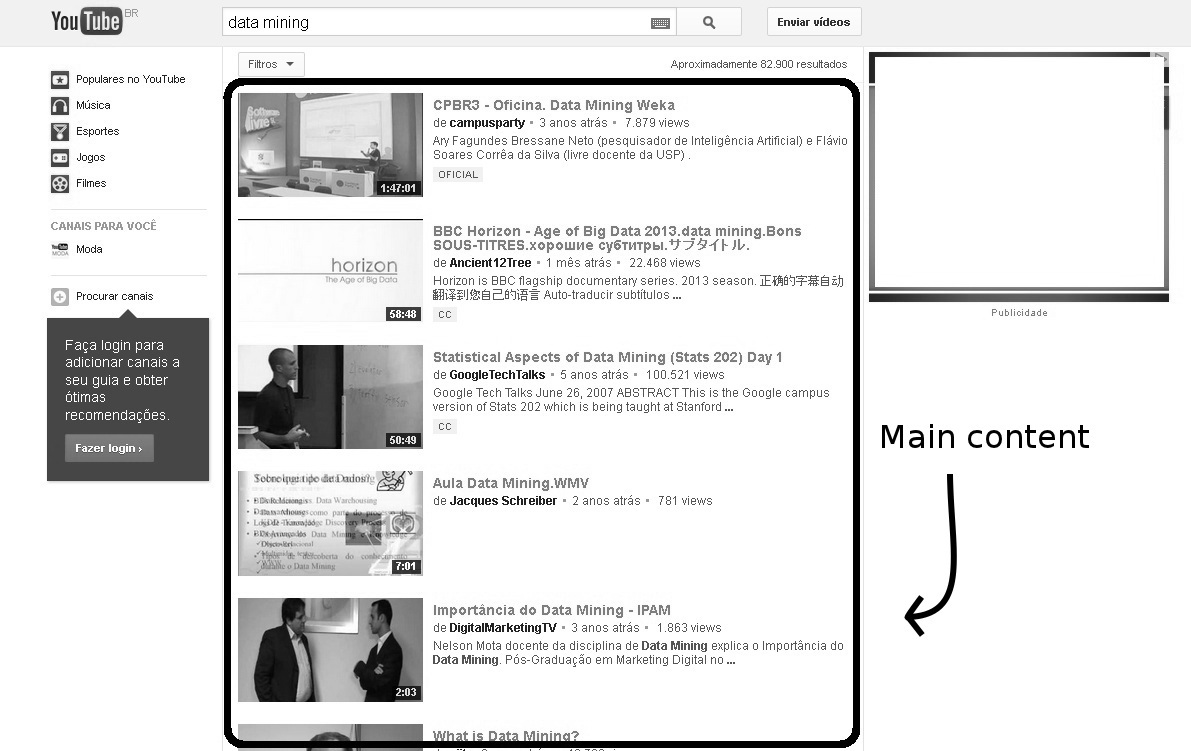
\includegraphics[scale=0.26]{example2-gs.jpg}
  \caption{A page from the YouTube web site and the main content region delimited.}
  \label{fig:ex2}
\end{figure}

\begin{figure}[H]
  \centering
    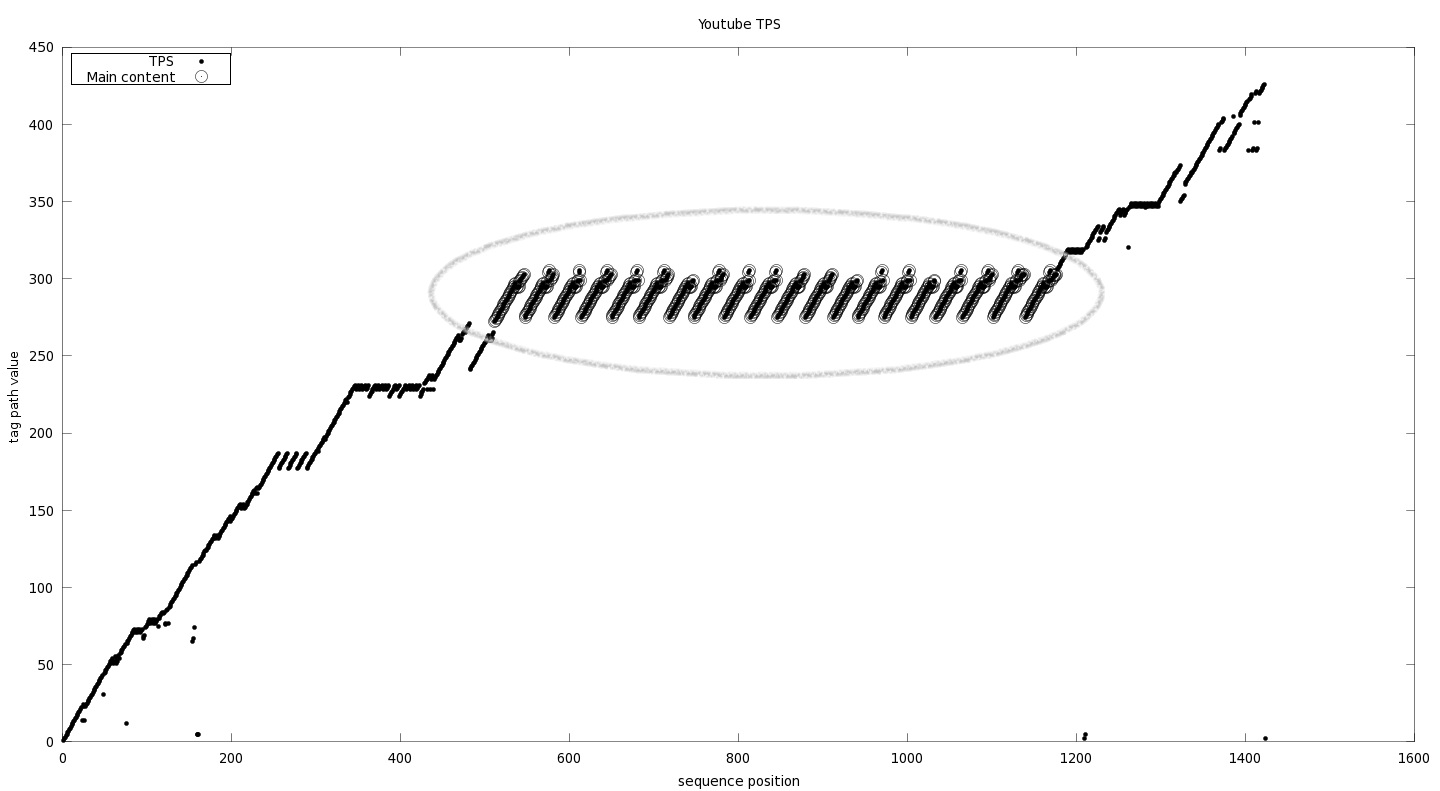
\includegraphics[scale=0.22]{tps.jpg}
  \caption{The TPS from a YouTube web page and the detected main content region.}
  \label{fig:tps}
\end{figure}


Without applying TPS filtering, we get $82$ records in total and, since we know
there are $20$ target records in this page, we can consider the value of $62$ 
records to be $100\%$ of noise to be removed. When we use TPS filtering, this 
time we get only the $20$ target records in the extraction phase, yielding a 
precision of $100\%$, that means all noise was removed in this case. We calculate 
the percentage of noise removed to be
\begin{equation}\label{eq:noise}
NoiseRemoved=1-\frac{\#Rec_{totalTPS}-\#Rec_{targetTPS}}{\#Rec_{total}-\#Rec_{target}}
\end{equation}
Where $\#Rec_{total}$ and $\#Rec_{target}$ are the total number of records and the
number of target records, respectively, from the original web page, and $\#Rec_{totalTPS}$ 
and $\#Rec_{targetTPS}$ are the total number of records and the number of target records, 
respectively, from the filtered web page.

\subsection{Results}\label{sub:res}

In Table \ref{table:results} we present, in the first three columns, the size of the DOM tree
processed by MDR and the reduction obtained after filtering. The column ``Content Present''
indicates whether or not the filtering process preserved the main content region. The next 
four columns are the results of MDR alone and combined with TPS filtering, showing the total 
records and target records extracted for both approaches. The last column shows the percentage 
of noise removed, calculated using Equation \ref{eq:noise}.  

As we can see in Table \ref{table:results}, the total of column ``Content
Present'' indicates that the algorithm has worked in 86.96\% of the sites and it
has removed, for this test set, an average of 77.03\% of all noise present in the
data, as shown by the average of column ``Noise rem.". We consider these to be
good results.

The average DOM tree reduction of 46.22\% is an interesting result. First,
because that means almost half the DOM tree is noise in average. Second, because
this number matches the value reported, independently, by \cite{Volume05} as
page template size (between $40\%$ and $50\%$), corroborating with literature work.

An interesting situation we can see in Table \ref{table:results} is the result
for the site ``g1.com.br''. Without filtering, MDR has reported a total of $225$
records, included $10$ target records. After filtering is applied, a total of
$202$ records are reported, none of them targets, all noise. So, after filtering, if
we had reported the complementary DOM tree instead, we would get a result of
$23$ records in total ($202-225=23$), included here the $10$ target records, which
is an excellent result since it gives us a $93.99\%$ of noise removal. We can 
deduce from this, that the segmentation has worked just fine for this site, only 
the main content was not correctly identified, since it's relatively small.

\subsection{Results Discussion}

There are three main situations where the algorithm needs to be improved but, fortunately, 
only two of these can lead to loss of main content (content removal). In Table
\ref{table:results}, column ``Content Present'', these two situations account for 13.04\% 
of the cases, where the content region was removed in the filtering process.

\begin{enumerate}
  \item{\textbf{templates too homogeneous}}. These are pages with little difference between
  the regions. In this case, using this technique, there is
  not much to do. We simply do not have enough information to work with,
  since the entire page looks alike. We do not lose the target records, but the
  amount of noise removed is very low;
  \item{\textbf{templates too heterogeneous}}. These are pages where the main content is 
  subdivided in more than one region. In this case, the main region gets split
  over and over, and only the largest part passes through the filter (and it
  might be noise). We propose a way to work around this problem later in this Section;
  \item{\textbf{pages where the main content is smaller than the rest}}. That is a
  consequence of the second assumption we made in Section \ref{sec:probform}:
  ``the main region is denser/bigger than the rest''. In this case, noise will
  always be reported as content. The same proposal made for the former situation 
  can be used to deal with this one as well.
\end{enumerate}

In the case of heterogeneous templates, TPS filtering can still be used if we
make some slight modifications in the algorithm. One such case of heterogeneous
template are ``news sites'', where every record has a different structure, but
they are all records from the same domain (i.e. they belong to the same entity). 
In this specific situation, TPS segmentation could be used to split the page in 
several parts, and a semantic approach used to combine the regions, reporting the
main content as a set of regions instead of only one.

For situation described for the site ``g1.com.br'' (that happened for two other
sites we tested), when the content region is smaller than the rest, we
could apply a semantic technique to check whether or not the desired content is
present in the reported region, if not, report the complementary DOM tree  (i.e.
inverse the pruning) instead. The main algorithm would look like this:

\begin{algorithm}[H]
\caption{Filters out noise from a web page}
\label{alg:tpsfilter2}
\textbf{Input:} $inputFile$ - an HTML file \\
\textbf{Output:} pruned $inputFile$'s DOM tree
\begin{algorithmic}[1]
\Procedure{tagPathSequenceFilter}{$inputFile$}
\State $DOMTree \leftarrow parseHTML(inputFile)$
\State $convertToSeq(DOMTree.body,$`` ''$,TPS)$
\State $backupTPS \leftarrow TPS$
\State $searchRegion(TPS)$
\If {$TPS$ not $content$}
\State $TPS = backupTPS - TPS$   
\EndIf
\State $pruneDOMTree(DOMTree.body,TPS)$
\State return $DOMTree$
\EndProcedure
\end{algorithmic}
\end{algorithm}

Algorithm \ref{alg:tpsfilter2} is the same as Algorithm \ref{alg:tpsfilter}, except for Line $6$
where it checks if the main content is present in the reported region and, if not, we report
the complementary sequence instead (Line $7$), ensuring the presence of the main content. 

\section{Conclusion}\label{sec:conclusion}

As shown in the results, the method we have proposed for page segmentation and noise
removal is very effective for some commercial/institutional web sites.
In most cases, a very large amount of noise is removed without compromising the
main content region. Also, when applied in conjunction with MDR, we can see that
the extraction precision is greatly improved.

In the situations where our algorithm fails, other techniques have to/should/could
be combined depending on the targeted application. In extreme cases, where a
page has either too homogeneous structure (so we can not find a split anywhere
along the TPS) or too heterogeneous structure (then the main content itself gets
split in several parts), the main content block could be detected using,
perhaps, semantic approaches.


%techniques, like the one presented in \cite{Adaptive07}, that labels a sequence 
%of blocks as $content$ or $notContent$ could be used to implement 
%line $6$ of algorithm \ref{alg:tpsfilter2}.

The algorithm shows outstanding performance, as it works very well for the majority 
of large commercial web sites we have tested. It also outcomes the limitations 
(training requirements, HTML tag dependency, manual labeling, among others) of previous 
works in the area of data cleaning, page segmentation and noise removal as mentioned in 
Section \ref{sec:relatedwork}.

% INCLUDE BIBLIOGRAPHY WHICH MUST FOLLOW jidm.bst TEMPLATE
\bibliographystyle{abbrv}
\bibliography{refs}  % sigproc.bib is the name of the Bibliography in this case
% You must have a proper ".bib" file
%  and remember to run:
% latex bibtex latex latex
% to resolve all references
%
% ACM needs 'a single self-contained file'!
%
%APPENDICES are optional
\balancecolumns

\appendix
\section{Compiled results}

\begin{table*}[h]
\centering
\caption{Compiled results}
\label{table:results}
\begin{tabular}{l r r r c r r r r r}

\hline\hline
\multicolumn{5}{c}{} & \multicolumn{4}{c}{MDR (\# records)} & (eq. \ref {eq:noise})\\
& \multicolumn{3}{c}{DOM size (\# nodes)} & Content & \multicolumn{2}{c}{Raw} &
\multicolumn{2}{c}{Pruned} & Noise\\
Site & Raw & Pruned & Reduction & present & Tot & Tgt & Tot & Tgt & rem.
\\
\hline
acm.org & 601 & 340 & -43.43\% & Yes & 61 & 10 & 16 & 10 & 88.24\% \\
amazon.com & 3309 & 1054 & -68.15\% & Yes & 368 & 15 & 27 & 15 & 96.60\% \\
americanas.com.br & 2660 & 710 & -73.31\% & Yes & 211 & 20 & 20 & 20 & 100.00\% \\
bestbuy.com & 3632 & 1425 & -60.77\% & Yes & 299 & 15 & 15 & 15 & 100.00\% \\
bondfaro.com.br & 3897 & 3069 & -21.25\% & Yes & 231 & 28 & 178 & 28 & 26.11\% \\
bradesco.com.br & 1913 & 1113 & -41.82\% & Yes & 164 & 10 & 93 & 10 & 46.10\% \\
buscape.com.br & 3608 & 3514 & -2.61\% & Yes & 279 & 24 & 266 & 24 & 5.10\% \\
ebay.com & 2623 & 1801 & -31.34\% & Yes & 162 & 50 & 50 & 50 & 100.00\% \\
elsevier.com & 906 & 160 & -82.34\% & Yes & 120 & 10 & 32 & 10 & 80.00\% \\
g1.com.br & 900 & 619 & -31.22\% & No & 225 & 10 & 202 & 0 & N/A \\
globo.com & 400 & 193 & -51.75\% & Yes & 80 & 10 & 20 & 10 & 85.71\% \\
google.com & 1421 & 981 & -30.96\% & Yes & 118 & 11 & 61 & 11 & 53.27\% \\
itau.com.br & 1111 & 410 & -63.10\% & No & 77 & 10 & 11 & 0 & N/A \\
magazineluiza.com.br & 3167 & 1115 & -64.79\% & Yes & 314 & 40 & 44 & 40 & 98.54\% \\
mercadolivre.com.br & 2401 & 1771 & -26.24\% & Yes & 136 & 50 & 52 & 50 & 97.67\% \\
reuters.com & 1202 & 480 & -60.07\% & Yes & 136 & 10 & 54 & 10 & 65.08\% \\
scopus.com & 4929 & 4688 & -4.89\% & Yes & 114 & 20 & 75 & 20 & 41.49\% \\
submarino.com.br & 2389 & 1268 & -46.92\% & Yes & 116 & 20 & 22 & 20 & 97.92\% \\
terra.com.br & 869 & 588 & -32.34\% & Yes & 122 & 50 & 76 & 50 & 63.89\% \\
valor.com.br & 514 & 126 & -75.49\% & No & 55 & 10 & 2 & 0 & N/A \\
webmotors.com.br & 2119 & 1361 & -35.77\% & Yes & 113 & 14 & 19 & 14 & 94.95\% \\
%wikipedia.com & 3224 & 1949 & -39.55\% & Yes & N/A & N/A & N/A & N/A & N/A \\
yahoo.com & 760 & 290 & -61.84\% & Yes & 67 & 10 & 10 & 10 & 100.00\% \\
youtube.com & 1424 & 674 & -52.67\% & Yes & 82 & 20 & 20 & 20 & 100.00\% \\
\hline
Average/Total &  &  & -46.22\% & 86.96\%&  &  &  &  & 77.03\% \\
  &  &  &  & 13.04\%&  &  &  &  &  \\
\hline

\end{tabular}
\end{table*}

\end{document}
